\documentclass[14pt]{beamer}

\usetheme{Montpellier}
\usecolortheme{beaver}

\usepackage{amsmath, amssymb, ../../vimacros, hyperref, tikz}
\usetikzlibrary{positioning, fit, bayesnet, shapes.misc}
\usepackage[round]{natbib}

\hypersetup{breaklinks=true, colorlinks=true, linkcolor=blue, urlcolor=blue, citecolor=blue}

\title{Discrete Variables in DGMs}
\author{Philip Schulz and Wilker Aziz\\
\url{https://github.com/philschulz/VITutorial}}
\date{}

\setbeamertemplate{footline}[frame number]

\begin{document}

\begin{frame}
\maketitle
\end{frame}

\begin{frame}{What we know so far}
\begin{itemize}
\item Deep Generative Models are probabilistic models where the parameters of the conditional
distributions are computed by neural networks
\pause
\item Because the $ \ELBO $ cannot be computed exactly, we need to sample latent values
\pause
\item Main problem: the MC estimator is not differentiable
\pause
\item Solution: reparametrisation gradient
\end{itemize}
\end{frame}

\begin{frame}{Reparametrisation Gradient}
\begin{block}{Model Gradient}
\begin{equation*}
\frac{\partial}{\partial \theta}\E[q(z|\lambda)]{\log p(x|z,\theta)} - \frac{\partial}{\partial \theta}\KL{q(z|\lambda)}{p(z|\theta)}
\end{equation*}
\end{block}
\pause
\begin{block}{Inference Network Gradient}
\begin{equation*}
\frac{\partial}{\partial \lambda}\E[q(z|\lambda)]{\log p(x|z,\theta)} - \frac{\partial}{\partial \lambda}\KL{q(z|\lambda)}{p(z|\theta)}
\end{equation*}
\end{block}
\end{frame}

\begin{frame}{Reparametrisation Gradient}
\begin{equation*}
\begin{aligned}
&\frac{\partial}{\partial \lambda}\E[q(z|\lambda)]{\log p(x|z,\theta)} &= \\
\pause
&\frac{\partial}{\partial \lambda}\E[\phi(\epsilon)]{\log p(x|\overbrace{h^{-1}(\epsilon, \lambda)}^{z},\theta)} &= \\
\pause
&\E[\phi(\epsilon)]{\frac{\partial}{\partial z}\log p(x|\overbrace{h^{-1}(\epsilon, \lambda)}^{z},\theta) \times \frac{\partial}{\partial \lambda}
\overbrace{h^{-1}(\epsilon, \lambda)}^{z}} &
\end{aligned}
\end{equation*}
\end{frame}

\begin{frame}
\tableofcontents
\end{frame}

\section{Reparametrisation for Discrete Variables?}
\begin{frame}
\tableofcontents[currentsection]
\end{frame}

\begin{frame}{Reparametrisation}
In order to tranform variables, we need to compute the Jacobian (matrix of derivatives).
\begin{equation*}
p(z) = \phi(h(z))\left|\frac{d}{dz}h(z)\right|
\end{equation*}
The Jacobian is generally not available for discrete variables. 
\end{frame}

\begin{frame}{Cumulative Distribution Function}
Insert picture here
\end{frame}

\begin{frame}{Continuity}
The outcome space of discrete variables is non-continuous. Thus, we cannot take derivatives with
respect to real variables. 
\end{frame}

\section{Revisiting the Inference Gradient}
\begin{frame}
\tableofcontents[currentsection]
\end{frame}

\begin{frame}
\begin{equation*}
\begin{aligned}
\frac{\partial}{\partial \lambda}&\E[q(z|\lambda)]{\log p(x|z,\theta)} = \\
\pause
\frac{\partial}{\partial \lambda}&\sum_{z} q(z|\lambda) \log p(x|z,\theta) = \\
\pause
&\sum_{z}\frac{\partial}{\partial \lambda} q(z|\lambda) \log p(x|z,\theta)
\end{aligned}
\end{equation*}
\end{frame}

\begin{frame}{Back to Basic Calculus}
\begin{equation*}
\frac{d}{d\lambda}\log f(\lambda) \pause = \frac{\frac{d}{d\lambda}f(\lambda)}{f(\lambda)}
\end{equation*}
\pause
\begin{block}{Consequence}
\begin{equation*}
\frac{d}{d\lambda}f(\lambda) = \frac{d}{d\lambda}\log f(\lambda) \times f(\lambda) 
\end{equation*}
\end{block}
\end{frame}

\begin{frame}{Score Function Estimator}
\begin{equation*}
\frac{d}{d\lambda}f(\lambda) = \frac{d}{d\lambda}\log f(\lambda) \times f(\lambda) 
\end{equation*}
\pause
Apply this to the ELBO derivative.
\begin{equation*}
\begin{aligned}
&\sum_{z}\frac{\partial}{\partial \lambda}q(z|\lambda)\log p(x|z,\theta) = \\
\pause
&\sum_{z}q(z|\lambda)\frac{\partial}{\partial \lambda}\log q(z|\lambda) \times \log p(x|z,\theta) = \\
\pause
&\E[q(z|\lambda)]{\frac{\partial}{\partial \lambda}\log q(z|\lambda) \times \log p(x|z,\theta)}
\end{aligned}
\end{equation*}
\end{frame}

\begin{frame}{Comparison Between Estimators}
\begin{itemize}
\item Score function gradient
\begin{equation*}
\E[q(z|\lambda)]{\frac{\partial}{\partial \lambda}\log q(z|\lambda) \times \log p(x|z,\theta)}
\end{equation*}
\item Reparametrisation gradient
\begin{equation*}
\E[\phi(\epsilon)]{\frac{\partial}{\partial \lambda} \log p(x|h^{-1}(\epsilon, \lambda),\theta)}
\end{equation*}
\end{itemize}
\end{frame}

\begin{frame}{Example Model}
Let us consider a latent factor model for topic modelling. Each document $ x $ consists of $ n $ i.i.d.
categorical draws from that model. The categorical distribution in turn depends on the binary latent 
factors $ z = (z_{1},\ldots,z_{k}) $ which are also i.i.d.
\begin{equation*}
\begin{aligned}
z_{j} &\sim \BerDist{\phi} && (1 \leq j \leq k) \\ 
x_{i} &\sim \CatDist{g(z)} && (1 \leq i \leq n)
\end{aligned}
\end{equation*} 
Here $ g(\cdot) $ is a function computed by neural network with softmax output.
\end{frame}

\begin{frame}{Example Model}
\begin{figure}
\center
\begin{tikzpicture}
\foreach \x in {1,...,4} {
  \pgfmathtruncatemacro{\y}{\x-1}
  \ifthenelse{\x=1}{\node[obs] (x\x) {$ x_{\x} $}}{\node[obs, right= of x\y] (x\x) {$ x_{\x} $}};
}
\foreach \z in {1,2,3} {
  \node[latent, above right = of x\z] (z\z) {$ z_{\z} $};
  \edge{z\z}{x1,x2,x3,x4};
}
\end{tikzpicture}
\end{figure}
At inference time the latent variables are marginally dependent. For our variational distribution
we are going to assume that they are not (recall: mean field assumption).
\end{frame}

\begin{frame}{Inference Network}
\begin{figure}
\center
\begin{tikzpicture}
\foreach \x in {1,...,4} {
\pgfmathtruncatemacro{\y}{\x-1}
\ifthenelse{\x=1}{\node[obs] (x\x) {$ x_{\x} $}}{\node[obs, right= of x\y] (x\x) {$ x_{\x} $}};
}
\foreach \z in {1,2,3} {
  \node[latent, above right = of x\z] (z\z) {$ z_{\z} $};
  \edge[color=red]{x1,x2,x3,x4}{z\z};
}
\end{tikzpicture}
\end{figure}
The inference network needs to predict $ k $ Bernoulli parameters $ \psi $. Any neural network with
sigmoid output will do that job.
\end{frame}

\begin{frame}{Computation Graph}
\begin{figure}
\center
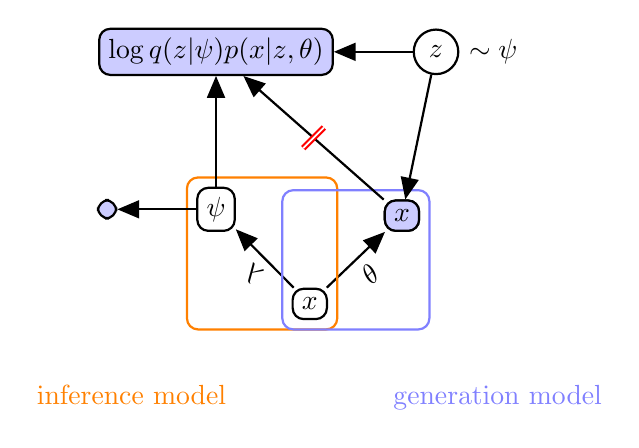
\begin{tikzpicture}[node distance=1cm]
\node[rectangle, draw, rounded corners, thick] (input) {$x$};
\node[rectangle, draw, rounded corners, thick, above left=of input] (psi) {$ \psi $};
\node[rectangle, fill=blue!20, thick, above right= of input, rounded corners, draw] (loss) {$ x $};
\draw[->, thick] (input) -- (psi) node[midway, above, rotate=145] {$ \lambda $};
\draw[->, thick] (input) -- (loss) node[midway, above, rotate=225] {$ \theta $};
\node[draw=orange, thick, rectangle, fit= (input) (psi), rounded corners] {};
\node[below left= of input] (inference) {\textcolor{orange}{inference model}};
\node[draw=blue!50, thick, rectangle, fit= (input) (loss), rounded corners] {};
\node[below right= of input] (generation) {\textcolor{blue!50}{generation model}};

\pause
\node[rectangle, draw, fill=blue!20, thick, rounded corners, thick, left=of psi] (kl) {$ \KullbackLeibler $};
\draw[->, thick] (psi) edge (kl);

\pause
\node[rectangle, fill=blue!20, thick, above of= psi, rounded corners, draw, node distance=2cm] (scorefunction) {$ \log q(z|\psi) p(x|z,\theta) $};
\node[rectangle, fill=blue!20, thick, above right= of input, rounded corners, draw] (loss) {$ x $};
\draw[->, thick] (psi) edge (scorefunction);
\draw[->, thick] (loss) edge node[strike out,draw,-,red,double]{} (scorefunction);

\pause
\node[circle, draw, thick, right= of scorefunction] (z) {$ z $};
\node[right = of z, xshift=-1cm] (random) {$ \sim \BerDist{\psi} $};
\draw[->, thick] (z) edge (loss);
\draw[->, thick] (z) edge (scorefunction);
\end{tikzpicture}
\end{figure}
\end{frame}

\begin{frame}{Reparametrisation Gradient}
\begin{figure}
\center
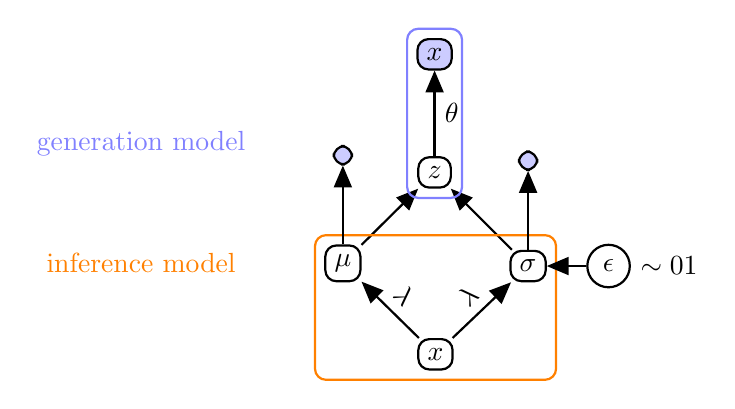
\begin{tikzpicture}[node distance=1cm]
\node[rectangle, draw, rounded corners, thick] (input) {$x$};
\node[rectangle, draw, rounded corners, thick, above left=of input] (mu) {$ \mu $};
\node[rectangle, draw, rounded corners, thick, above right=of input] (var) {$ \sigma $};
\node[rectangle, draw, rounded corners, thick, above right= of mu] (z) {$ z $};
\node[rectangle, fill=blue!20, thick, above of= z, rounded corners, draw, node distance=1.5cm] (output) {$ x $};

\draw[->, thick] (input) -- (mu) node[midway, above, rotate=315] {$ \lambda $};
\draw[->, thick] (input) -- (var) node[midway, above, rotate=45] {$ \lambda $};
\draw[->, thick] (mu) edge (z);
\draw[->, thick] (var) edge (z);
\draw[->, thick] (z) -- (output) node[midway, right] {$ \theta $};

\node[draw=orange, thick, rectangle, fit= (input) (mu) (var), rounded corners] {};
\node[left= of mu] (inference) {\textcolor{orange}{inference model}};

\node[draw=blue!50, thick, rectangle, fit= (z) (output), rounded corners] {};
\node[above= of inference] (generation) {\textcolor{blue!50}{generation model}};

\node[circle, draw, thick ,right =of var, xshift=-.5cm] (epsilon) {$ \epsilon $};
\node[right = of epsilon, xshift=-1cm] (stdNormal) {$ \sim \NDist{0}{1} $};
\draw[->, thick] (epsilon) edge (var);

\node[above= of mu, rectangle, draw, fill=blue!20, thick, rounded corners, thick] (KLmu) {$ \KullbackLeibler $};
\draw[->, thick] (mu) edge (KLmu);
\node[above= of var, rectangle, draw, fill=blue!20, thick, rounded corners, thick] (KLvar) {$ \KullbackLeibler $};
\draw[->, thick] (var) edge (KLvar);
\end{tikzpicture}
\end{figure}
\end{frame}

\begin{frame}{Pros and Cons}
\begin{itemize}
\item Pros
\begin{itemize}
\item Applicable to all distributions
\item Many libraries come with samplers for common distributions
\end{itemize}
\pause
\item Cons
\begin{itemize}
\item High Variance!
\end{itemize}
\end{itemize}
\end{frame}

\section{Control Variates and Baselines}

\begin{frame}
\tableofcontents[currentsection]
\end{frame}

\begin{frame}{Baselines}
We attempt to centre the gradient estimate. To do this we learn a quantity $ C $ that we subtract
from the reconstruction loss.
\begin{equation*}
\log q(z|\lambda) \left( p(x|z,\theta) - C \right)
\end{equation*}
We call $ C $ a baseline. It does not change the expected gradient \citep{Williams:1992}.
\end{frame}

\begin{frame}{Baselines}
We can make baselines input-depdendent to make them more flexible.
\begin{equation*}
\log q(z|\lambda) \left( p(x|z,\theta) - C(x) \right)
\end{equation*}
However, baselines may not depend on the random value $ z $! Quantities that may depend on the
random value ($ C(z) $) are called \textbf{control variates}. See \cite{PaisleyEtAl:2012, RanganathEtAl:2014,GregorEtAl:2014}.
\end{frame}

\begin{frame}{Baselines}
Baselines are predicted by a regression model (e.g. a neural net). The model is trained using 
an $ L_{2} $-loss.
\begin{equation*}
\min \left(C(x) - p(x|z,\theta)\right)^{2}
\end{equation*}
\end{frame}

\begin{frame}{Summary}
\begin{itemize}
\pause
\item Reparametrisation not available for discrete variables.
\pause
\item Use score function estimator.
\pause
\item High variance.
\pause
\item Always use baselines for variance reduction!
\end{itemize}
\end{frame}

\begin{frame}[allowframebreaks]
\bibliographystyle{plainnat}
\bibliography{../../VI}
\end{frame}

\end{document}